\documentclass[a4paper, 18pt]{article}
\usepackage[T1]{fontenc}
\usepackage[portuguese]{babel}
\usepackage[utf8]{inputenc}
\usepackage[margin=2cm,includefoot,footskip=30pt,]{geometry}

\usepackage{graphicx}
\graphicspath{ {imagens/} }
\usepackage{bold-extra}
\usepackage{epstopdf}
\usepackage{float}
\usepackage{scalerel}
\usepackage{enumerate}
\usepackage{indentfirst}
\usepackage{mathtools}
\usepackage{amsmath}
\allowdisplaybreaks
\usepackage{cleveref}
\usepackage{amssymb}
\usepackage{listings}
\usepackage{color}
\newcommand\showdiv[1]{\overline{\smash{\hstretch{.5}{)}\mkern-3.2mu\hstretch{.5}{)}}#1}}
\newcommand\ph[1]{\textcolor{white}{#1}}


\definecolor{dkgreen}{rgb}{0,0.6,0}
\definecolor{gray}{rgb}{0.5,0.5,0.5}
\definecolor{mauve}{rgb}{0.58,0,0.82}
\definecolor{mygreen}{RGB}{28,172,0} % color values Red, Green, Blue
\definecolor{mylilas}{RGB}{170,55,241}

%\lstset{language=Matlab,%
%    %basicstyle=\color{red},
%    breaklines=true,%
%    morekeywords={matlab2tikz},
%    keywordstyle=\color{blue},
%    morekeywords=[2]{1}, keywordstyle=[2]{\color{black}},
%    identifierstyle=\color{black},
%    stringstyle=\color{mylilas},
%    commentstyle=\color{mygreen},
%    showstringspaces=false,
%	%inputencoding=utf8,
%	extendedchars=true,
%	literate={á}{{\'a}}1 {ã}{{\~a}}1 {â}{\^{a}}1 {é}{\'{e}}1 {ç}{\c{c}}1 {ã}{\~{a}}1 {à}{\`{a}}1 {ê}{\^{e}}1 {í}{\'{i}}1 {ó}{\'{o}}1 {õ}{\~{o}}1 {ô}{\^{o}}1 {ú}{\'{u}}1 {Ç}{\c{C}}1,
%}


\lstset{frame=tb,
  language=Matlab,
  aboveskip=3mm,
  belowskip=3mm,
  showstringspaces=false,
  columns=flexible,
  basicstyle={\small\ttfamily},
  numbers=none,
  numberstyle=\tiny\color{gray},
  keywordstyle=\color{blue},
  commentstyle=\color{dkgreen},
  stringstyle=\color{mauve},
  breaklines=true,
  breakatwhitespace=true,
  tabsize=3,
  extendedchars=true,
  literate=	{á}{{\'a}}1	{ã}{{\~a}}1	{â}{\^{a}}1	{é}{\'{e}}1	{ç}{\c{c}}1
  			{ã}{\~{a}}1	{à}{\`{a}}1 {ê}{\^{e}}1 {í}{\'{i}}1	{ó}{\'{o}}1
  			{õ}{\~{o}}1 {ô}{\^{o}}1	{ú}{\'{u}}1 {Ç}{\c{C}}1,
}

% ----- Cabeçalho e rodapé -----
\usepackage{fancyhdr}
\pagestyle{fancy}
\fancyhf{}

\renewcommand{\headrulewidth}{1pt}
\renewcommand{\footrulewidth}{0.5pt}

\rhead{1º Trabalho Computacional}
\lhead{Matemática Computacional\rightmark}
\rfoot{Página \thepage}
\lfoot{\small Engenharia Eletrotécnica e de Computadores - IST}


\usepackage{pdfpages}

\begin{document}


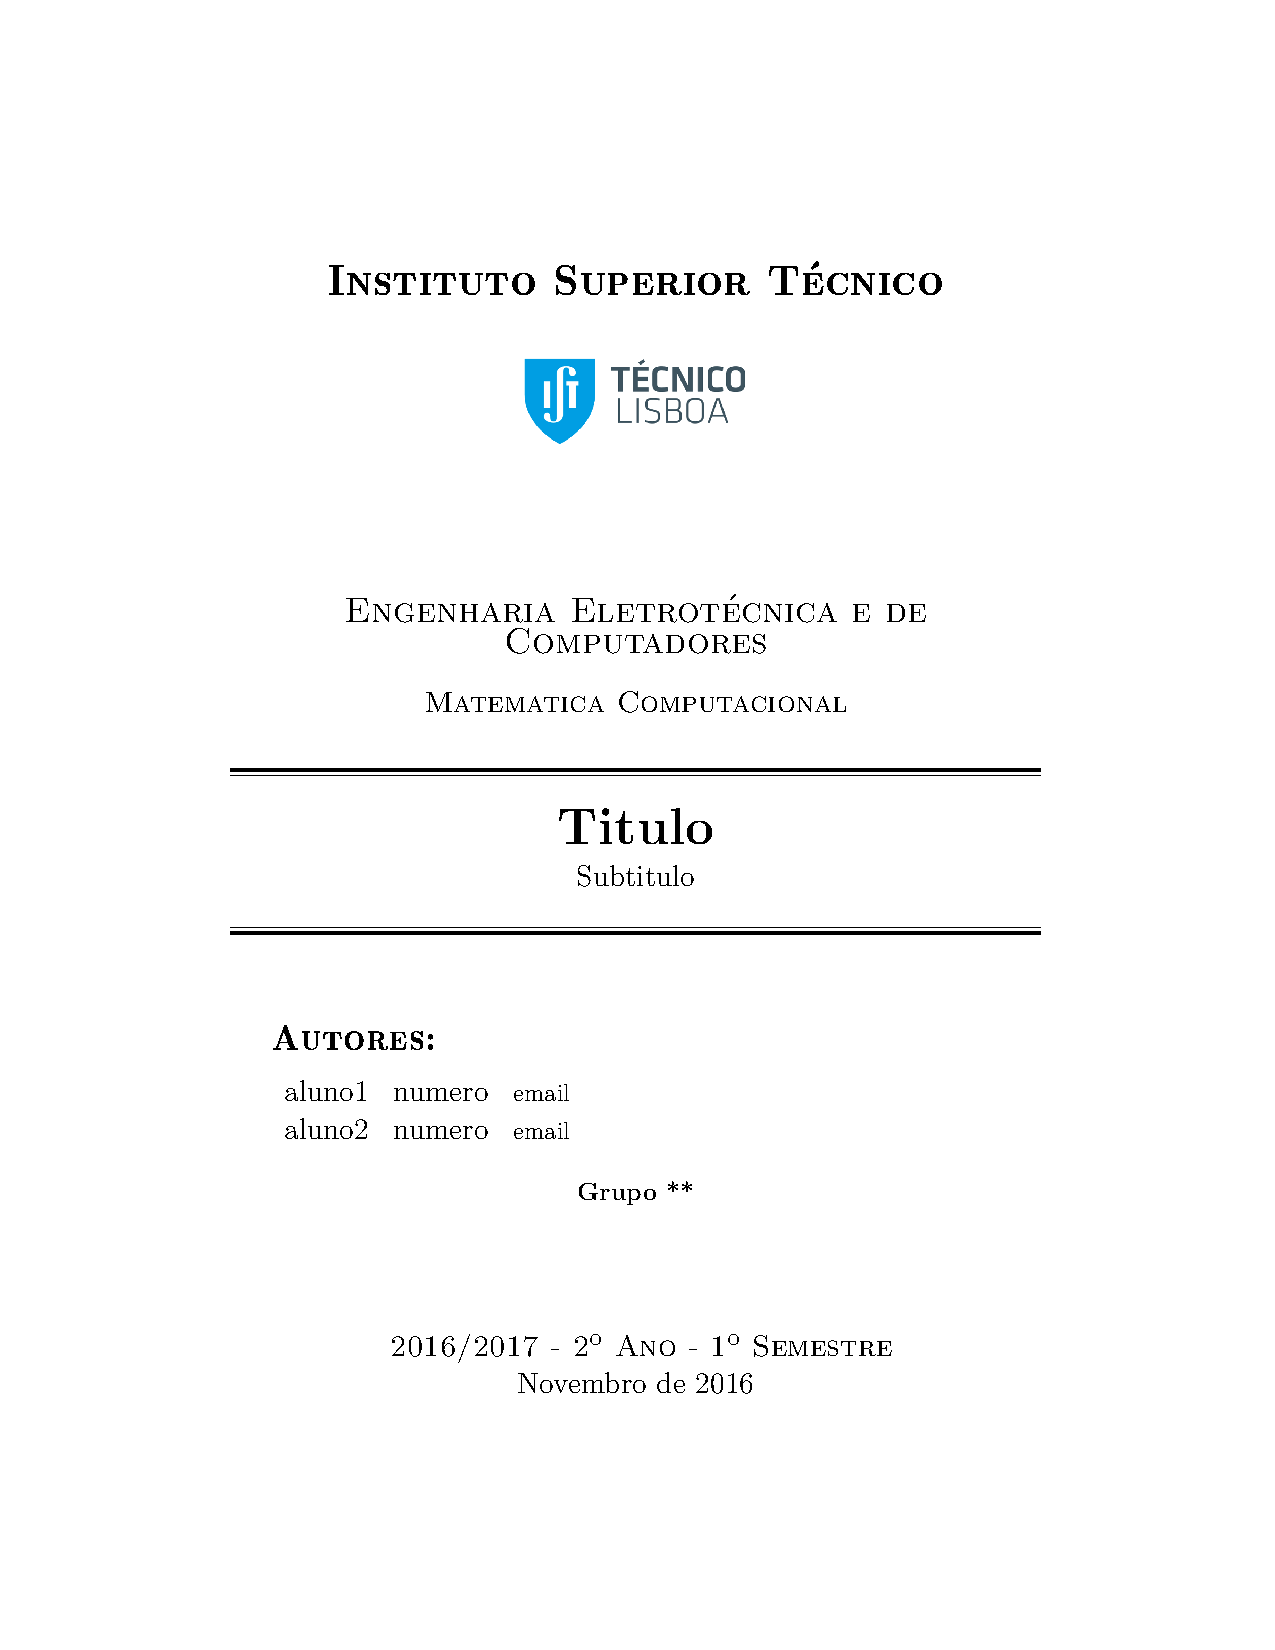
\includepdf[pages={1}]{capa/capa.pdf}

\section{Pergunta 1}
	\begin{equation} \label{init}
		h(\lambda) = \lambda + 15.5 - 2\cosh(\lambda\tau)
	\end{equation}

	$$h'(\lambda) = 1 - 2\sinh(\tau\lambda) = 1 - \tau(e^{\tau\lambda} - e^{-\tau\lambda})$$

	$$h''(\lambda) = -2\tau^2\cosh(\tau\lambda) = -\tau^2(e^{\tau\lambda} + e^{-\tau\lambda})$$

	\par
	Analisemos o sinal de $h''(\lambda)$:
	$$\tau > 0$$
	\begin{equation} \label{eq:1_2nd_der_sign}
	\begin{split}
		e^{\tau\lambda} + e^{-\tau\lambda} > 0 &\implies h''(\lambda) < 0, \forall \lambda
	\end{split}
	\end{equation}

	\par
	Pelo Teorema de Rolle e pela inequação \eqref{eq:1_2nd_der_sign} podemos afirmar que
	$h(\lambda)$ tem no máximo duas raízes. Provemos que $h(\lambda)$ tem no mínimo duas raízes sem perda de generalidade.

	$$h(0) = 0 + 15.5 - 2\cosh(0\tau) = 13.5 > 0$$

	\begin{align*}
		\lim_{x \to +\infty} h(\lambda)
		&= \lim_{x \to +\infty} (\lambda + 15.5 - 2\cosh(\lambda)) \\
		&= \lim_{x \to +\infty} e^{\tau\lambda} \bigg(\frac{\lambda}{e^{\tau\lambda}} + \frac{15.5}{e^{\tau\lambda}} - \frac{2\cosh(\lambda)}{e^{\tau\lambda}}\bigg) \\
		&= e^{+\infty} (0 + 0 - 1) = -\infty < 0
	\end{align*}

	\par
	Analogamente para  $-\infty$ :

	\begin{align*}
		\lim_{x \to -\infty} h(\lambda)
		&= \lim_{x \to -\infty} (\lambda + 15.5 - 2\cosh(\lambda)) \\
		&= \lim_{x \to -\infty} e^{-\tau\lambda} \bigg(\frac{\lambda}{e^{-\tau\lambda}} + \frac{15.5}{e^{-\tau\lambda}} - \frac{2\cosh(\lambda)}{e^{-\tau\lambda}}\bigg) \\
		&= e^{+\infty} (0 + 0 - 1) = -\infty < 0
	\end{align*}

	\par
	% explicar melhor teorema de Bolzano
	Assim, como $h(\lambda)$ é contínua, pelo teorema de Bolzano conclui-se que $h(\lambda)$ tem no mínimo duas raízes, uma positiva e uma negativa. Logo, como $h(\lambda)$ tem no máximo duas raízes, tem exatamente duas raízes.
	\par
	Se $\tau = 0$:
	\begin{align*}
		h(\lambda) &= \lambda + 13.5 = 0 \Leftrightarrow \\
		\Leftrightarrow h &= -13.5
	\end{align*}

	\par
	Por outro lado, se $\tau$ for muito grande, existirá sempre um $\lambda$ arbritariamente perto de $0^-$ tal que:

	\begin{align*}
		\lambda + 15.5 &= 2cosh(\lambda\tau) \Leftrightarrow \\
		\Leftrightarrow h(\lambda) &= 0, \lambda < 0
	\end{align*}

	\par
	Assim, a raiz negativa estará contida no intervalo $]-13.5, 0[, \forall \tau > 0$.


\section{Pergunta 2}
\subsection*{a)}
	\begin{equation} \label{2a}
	\begin{split}
		g(\lambda) &= \lambda - 0.1(\lambda + 15.5 - 2cosh(0.8\lambda)) \Leftrightarrow \\
		\Leftrightarrow g(\lambda) &= 0.9\lambda - 1.55 + 0.2cosh(0.8\lambda)
	\end{split}
	\end{equation}

	\par
	A raiz positiva $z_2$ de \eqref{init} equivale a um ponto fixo de \eqref{2a} e será do tipo repulsor sse:
	$$|g'(z_2)| > 1$$

	\par
	Analisemos as derivadas da função iteradora $g(\lambda)$:
	$$g'(\lambda) = 0.9 + 0.16sinh(0.8\lambda)$$

	\begin{equation} \label{2a_2nd_der}
		g''(\lambda) = 0.128cosh(0.8\lambda) > 0, \forall \lambda
	\end{equation}

	% lambda pertence a r
	\par
	De \eqref{2a_2nd_der} vem que $g'(\lambda)$ é estritamente crescente e que $g(\lambda)$ tem a concavidade virada para cima, $\forall \lambda$.

	%\begin{align*}
	%	g(0) &< 0 \\
	%	g'(0) &> 0 \\
	%	g''(0) &\neq 0
	%\end{align*}

	% Explicação alternativa
	%\par
	%Em $\lambda = 0$ a função iteradora $g(\lambda)$ é negativa, mas a sua derivada já é positiva. Como a segunda derivada é sempre positiva, concluímos que $g(\lambda)$ em $\lambda = 0$ já está a crescer e continuará assim $\forall \lambda > 0$.
	%\par
	%Como a função é negativa nesse ponto, conclui-se que a única maneira de $g(\lambda)$ intersetar a reta $y = x$ (e assim ter um ponto fixo positivo $z_2$ raiz da equação \eqref{init}) é se ultrapassar o ritmo de crescimento da reta $y = x$, ou seja, se $g'(\lambda) > 1$ para algum $\lambda_0$ tal que $0 < \lambda_0 < z_2$. Como $g'(\lambda)$ é estritamente crescente, para $\lambda \geqslant \lambda_0$ então $g'(\lambda) > 1 $. Deste modo, o ponto fixo $z_2$ será repulsor.

	% Explicação do Morais
	\par
	\vspace{.5cm}
	Para $\lambda > 0$, temos as seguintes condições:

	\begin{align*}
		|g'(\lambda)| &> 1 \Leftrightarrow \\ &\Leftrightarrow
		(g'(\lambda) < -1 \vee g'(\lambda) > 1) \wedge \lambda > 0 \Leftrightarrow \\ &\Leftrightarrow
		(\lambda < \lambda_1 \vee \lambda > \lambda_2) \wedge \lambda > 0 \stepcounter{equation}\tag{\theequation}\label{2a_cond}
	\end{align*}

	\par
	Calculemos os pontos $\lambda_1$ e $\lambda_2$ que satisfaçam as condições em \eqref{2a_cond}.

	\begin{align*} % split não permite page breaks
		g'(\lambda_1) &= -1 \Leftrightarrow \\ &\Leftrightarrow
		0.9 + 0.16sinh(0.8\lambda_1) = -1 \Leftrightarrow \\ &\Leftrightarrow
		0.08(e^{0.8\lambda_1} - e^{-0.8\lambda_1}) = -1.9 \Leftrightarrow (w = e^{0.8\lambda_1}) \\ &\Leftrightarrow
		w - w^{-1} = \frac{-1.9}{.08} = -23.75 \Leftrightarrow \\ &\Leftrightarrow
		w.w - 23.75.w - w^{-1}.w = 0 \Leftrightarrow \\ &\Leftrightarrow
		w^2 + 23.75w - 1 = 0 \Leftrightarrow \\ &\Leftrightarrow
		w = \frac{-95 + \sqrt{9089}}{8} \vee w = \frac{-95 - \sqrt{9089}}{8} \Leftrightarrow \\ &\Leftrightarrow
		w \approx 0.04203 \vee w \approx -23.792 \text{  (impossível, $w = e^{0.8\lambda_1}$)} \Leftrightarrow \\ &\Leftrightarrow
		e^{0.8\lambda_1} = \frac{\sqrt{9089} - 95}{8} \Leftrightarrow \\ &\Leftrightarrow
		\lambda_1 = \frac{ln(\frac{\sqrt{9089} - 95}{8})}{0.8} \Leftrightarrow \\ &\Leftrightarrow
		\lambda_1 \approx -3.96169 \stepcounter{equation}\tag{\theequation}\label{lambda1}
	\end{align*}


	\begin{align*}
		g'(\lambda_2) &= 1 \Leftrightarrow \\ &\Leftrightarrow
		0.9 + 0.16sinh(0.8\lambda_2) = 1 \Leftrightarrow \\ &\Leftrightarrow
		0.16 * \frac{1}{2}(e^{0.8\lambda_2} - e^{-0.8\lambda_2}) = 0.1 \Leftrightarrow \\ &\Leftrightarrow
		w - w^{-1} = \frac{0.1}{0.08} = 1.25 \Leftrightarrow \\ &\Leftrightarrow
		w.w - 1.25.w - w^{-1}.w = 0 \Leftrightarrow \\ &\Leftrightarrow
		w^2 - 1.25w - 1 = 0 \Leftrightarrow \\ &\Leftrightarrow
		w = \frac{5 + \sqrt{89}}{8} \vee w = \frac{5 - \sqrt{89}}{8} \Leftrightarrow \\ &\Leftrightarrow
		w \approx 1.804 \vee w \approx -0.554 \text{  (impossível, $w = e^{0.8\lambda_2}$)} \Leftrightarrow \\ &\Leftrightarrow
		e^{0.8\lambda_2} = \frac{5 + \sqrt{89}}{8} \Leftrightarrow \\ &\Leftrightarrow
		\lambda_2 = \frac{ln(\frac{5 + \sqrt{89}}{8})}{0.8} \Leftrightarrow \\ &\Leftrightarrow
		\lambda_2 \approx 0.73786 \stepcounter{equation}\tag{\theequation}\label{lambda2}
	\end{align*}

	\par
	Completando as condições em \eqref{2a_cond} com \eqref{lambda1} e \eqref{lambda2}:

	\begin{align*}
		&|g'(\lambda)| > 1 \Leftrightarrow \\ \Leftrightarrow
		&(\lambda < -3.96169 \vee \lambda > .073768) \wedge \lambda > 0 \Leftrightarrow \\ \Leftrightarrow
		&\lambda > .073768
	\end{align*}

	\par
	Assim, para provar que o ponto fixo $z_2$ é repulsor, basta-nos provar que $z_2 > \lambda_2$.

	\begin{equation} \label{2a_bolz}
	\begin{split}
		&f(\lambda) = \lambda + 15.5 - 2cosh(0.8\lambda) \\
		&f(0) = 13.5 \\
		&f(\lambda_2) = f(.073768) \approx 13.215272
	\end{split}
	\end{equation}

	\par
	% TODO: podemos utilizar f() [usada originalmente pelo Morais] ou g()
	% TODO: incluir gráficos?
	Recorrendo ao Teorema de Bolzano, de \eqref{2a_bolz} sai que o ponto fixo $z_2$ tem que ser maior que $\lambda_2$, pois nesse ponto a função $g(\lambda)$ ainda se encontra abaixo da reta $y = x$. Sabemos que $z_2$ não pode pertencer ao intervalo $[0, \lambda_2]$ porque pelas suas derivadas se $\lambda > 0$ então $g(\lambda)$ é estritamente crescente.

\subsection*{b)}
	\par
	Analogamente a 2.a), se encontrarmos um intervalo $I$ para $\lambda < 0$ tal que $|g'(\lambda)| < 1, \forall \> \lambda \in I \wedge \lambda_0 \in I$, sabemos que o método do ponto fixo começando em $\lambda_0$ vai convergir para a raiz negativa $z_1$, sendo este um ponto fixo atrator.

	\par

	\begin{align*}
		|g'(\lambda)| &< 1 \Leftrightarrow \\ &\Leftrightarrow
		(g'(\lambda) > -1 \wedge g'(\lambda) < 1) \wedge \lambda < 0 \Leftrightarrow \\ &\Leftrightarrow
		(\lambda > \lambda_1 \wedge \lambda < \lambda_2) \wedge \lambda < 0 \\ &\Leftrightarrow
		(\lambda > -3.96169 \wedge \lambda < .073768) \wedge \lambda < 0  \stepcounter{equation} \\ &\Leftrightarrow
		0 < \lambda < -3.96169 \tag{\theequation}
	\end{align*}

	Desta inequação resulta que no intervalo $[\lambda_1, 0] = I$:
		$$|g'(\lambda)| < 1, \forall \> \lambda \in I$$

	\par
	Assim, resta provar que $g(\lambda)$ tem um ponto fixo no intervalo $I$, ou seja, interseta a reta $y = x$ para algum $\lambda \in I$.

	\begin{align*}
		g(0) &< 0 \\
		g(\lambda_1) = g(-3.96169) &\approx -2.6926708
	\end{align*}

	Claramente $\lambda_0 = -3 \in I$. Como $\lambda_1 > g(\lambda_1)$, este ponto econtra-se na região $y > x$, ou seja, à "esquerda" da reta $y = x$. Como $g(0) < 0$, este ponto encontra-se na região $y < x$, ou seja, à "direita" da reta $y = x$. Como $g(\lambda)$ é contínua, garante-se que esta função interseta a reta $y = x$ para $\lambda \in I$, logo, tem um ponto fixo atrator no intervalo $I$ e o método do ponto fixo $g(\lambda)$ converge para a raiz negativa $z_1$ começando em $\lambda_0 = -3$.

\subsection*{c)}
	Programa em anexo.

\subsection*{d)}
	\begin{table}[H]
		\setlength{\tabcolsep}{0.5cm} %padding das colunas
		\renewcommand{\arraystretch}{1.5} %padding das linhas
		\centering
		\caption{Iteradas do método do ponto fixo \eqref{2a}}
		\label{2d_table}
		\begin{tabular}{|c|c|c|}
			$n$ & $\lambda _n$ &  $| \lambda _{n+1} - \lambda _n |$ \\\hline
			0& -3.000000000000000 & 0.138610566606898 \\
			1& -3.138610566606898 & 0.003567390881155 \\
			2& -3.135043175725743 & 0.000275972711746 \\
			3& -3.135319148437489 & 0.000020989504121 \\
			4& -3.135298158933368 & 0.000001598504606 \\
			5& -3.135299757437974 & 0.000000121725579 \\
			6& -3.135299635712395 & - \\
		\end{tabular}
	\end{table}

\subsection*{e)}
	\subsubsection*{i.)}

	%formula da ordem de convergência

	\begin{table}[H]
		\setlength{\tabcolsep}{0.5cm} %padding das colunas
		\renewcommand{\arraystretch}{1.5} %padding das linhas
		\centering
		\caption{Sucessão de erros para ordem de convergência $p = \frac{1}{2}, 1, 2$}
		\label{2e_table}
		\begin{tabular}{|c|c|c|c}
			$n$ & $\frac{|e_{n+1}|}{|e_n|^{\frac{1}{2}}}$ &  $\frac{|e_{n+1}|}{|e_n|^1}$ & $\frac{|e_{n+1}|}{|e_n|^2}$ \\\hline
			0 & 0.009001228832727 & 0.024471099844949 & 0.000180865969935e3 \\
			1 & 0.009001228832727 & 0.024471099844949 & 0.000180865969935e3 \\
			2 & 0.004457019736082 & 0.077458574287344 & 0.023394802475624e3 \\
			3 & 0.001218451139231 & 0.076084871362003 & 0.296673459104577e3 \\
			4 & 0.000334315531198 & 0.075682869509848 & 3.878641714344468e3 \\
		% TODO: na última linha fica x_6 - x_6 = 0. é suposto ficar assim?
		\end{tabular}
	\end{table}

	\par
	A sucessão de erros que parece convergir para um $K_\infty > 0$ é a coluna de ordem de convergência $p = 1$.

	% o último termo da sucessão de erros de p = 1 fica mais diferente
	% de este resultado. Eu mexi no sucessao_de_erros.m para incluir mais
	% termos (são 6 e antes dava 5) e ainda por cima os primeiros dois eram iguais.
	% fodi alguma coisa?
	% METER FORMULA FIM PAG. 46/INC 47

\subsubsection*{ii.)}
	\par
	O valor teórico de $K_\infty$ é:

	$$K_\infty = |g'(\lambda_n)| = 0.076150166$$

	\par
	O que está perto da aproximação obtida em i), $0.075682869509848$.

\subsection*{f)}
	\par
	Para $\alpha = -0.02$:
	$$g'(-3) = 0.8125$$.

	\par
	Para $\alpha = -0.1$:
	$$g'(-3) = 0.0254$$

	No primeiro caso, a derivada em $\lambda = -3$ é superior. Logo, a convergência para $\alpha = -0.02$ será mais rápida ($K_\infty$ será menor).


\section{Pergunta 3}
\subsection*{a)}
	\begin{table}[H]
		\setlength{\tabcolsep}{0.5cm} %padding das colunas
		\renewcommand{\arraystretch}{1.5} %padding das linhas
		\centering
		\caption{Iteradas do método de Newton para \eqref{init} com $\tau = 0.8$}
		\label{}
		\begin{tabular}{|c|c|c|}
			$n$ & $\lambda _n$ &  $| \lambda _{n+1} - \lambda _n |$ \\\hline
			0 & 3.000000000000000  & 0.953542135177649  \\
			1 & 2.046457864822351  & 4.12986183157042 \\
			% TODO: Isto tá certo?... 2 e depois 6 e depois 5?
   			2 & 6.176319696392767  & 1.06598950585173 \\
   			3 & 5.110330190541037  & 0.836111134113811 \\
   			4 & 4.274219056427226  & 0.461638476296785 \\
   			6 & 3.812580580130441  & 0.116772305881346 \\
   			7 & 3.695808274249095  & 0.00624264760568893 \\
   			8 & 3.689565626643406  & 1.68277560947949e-05 \\
   			9 & 3.689548798887311  & 1.21873178215992e-10 \\
   			10 & 3.689548798765438 & - \\
		\end{tabular}
	\end{table}

	\par
	O método de Newton convergiu para a raiz positiva, a partir da aproximação inicial $x_0 = 3$ em 9 iterações.

\subsection*{b)}
	\par
	O método de Newton converge se forem cumpridas condições suficientes para a sua convergência.

	\par
	É necessário que num intervalo haja uma raiz (i), que seja única (ii) e não haja inversões de concavidades (iii),
	percebe-se porquê pensando no funcionamento geométrico do método - havendo inversão de concavidade, pode
	acontecer que as retas tangentes vão começar a fazer o método tender para outra raiz ou para qualquer outro sítio inesperado.

	Neste caso, apenas precisamos de provar a convergência para um ponto, pelo o que verificar que os extremos do intervalo também são convergentes é desnecessário. Assim, é apenas preciso verificarem-se as seguintes condições para o ponto:

	\begin{enumerate}[i)]
	\item $h(a)*h(b) < 0$, em que a e b são os limites inferior e superior, respetivamente do intervalo.
	Escolhendo dois pontos, $x_1 = 2$ e $x_2 = 5$, tem-se $h(2) * h(5) \approxeq -421.1723 < 0 $, verificando-se a condição.

	\item $h'(x) \neq 0 \> \forall \> x \in I$. A função não pode ser constante, para qualquer x.
	A derivada da função a estudar é sempre maior que 0, ou seja, f(x) é crescente. Sendo a segunda derivada sempre maior que 0, a derivada também é crescente.

	\item $h''(x) \geqslant 0 \vee h''(x) \leqslant 0 \> \forall \> x \in I$, ou seja, a sentido da concavidade tem de ser constante no intervalo.
	Neste caso particular, sabemos que a segunda derivada é sempre positiva no intervalo, concluindo-se que também esta condição se verifica.
	\end{enumerate}

	Escolhamos, ao acaso, o ponto $x = 3$. $h(3) \aprox 7.38611 > 0$, logo há convergência para esse ponto.

	A ordem de convergência também pode ser determinada rapidamente, descobrindo qual a primeira derivada que não se anula no intervalo. Sabemos desde já que a segunda derivada é sempre maior que 0, logo podemos concluir que este método, nestas condições e situação presente, tem convergência quadrática.

\section{Pergunta 4}
	\par Para uma aproximação inicial $\lambda _0 = 3$ e um $\alpha = 0.05$ obtem-se uma aproximação 3.689548652886207 do valor da raiz positiva $z_2$ em 13 iterações.
	
	O método de Newton vai convergir em menos iterações do que o método do ponto fixo, visto que a ordem de convergência do método de Newton é supralinear, enquanto o método do ponto fixo converge linearmente.


\section{Anexo}

\par{Ponto fixo}
	\lstinputlisting{../src/ponto_fixo.m}

\par{Metodo Newton}
	\lstinputlisting{../src/metodo_newton.m}

\end{document}
